\documentclass{beamer}
\usepackage{multicol,lipsum,caption}
\usepackage{mathtools, amsmath,booktabs,verbatim,tikz} 
\usetikzlibrary{shapes.geometric, arrows,positioning,matrix,calc}
%\usepackage{mathptmx}

\usetheme[progressbar=frametitle]{metropolis}
\setbeamertemplate{frame numbering}[fraction]
\useoutertheme{metropolis}
\useinnertheme{metropolis}
\usefonttheme{metropolis}
\usecolortheme{spruce}
\setbeamercolor{background canvas}{bg=white}

\title{Self-adaptative genetic algorithm for minimum thickness design of composite laminate}
\author{Huiyao Zhang}
\institute{Kyoto Institue of Technology}
\date{11-10-2020}
\setbeamertemplate{itemize/enumerate body begin}{\large}

\DeclarePairedDelimiter\Floor\lfloor\rfloor
\DeclarePairedDelimiter\Ceil\lceil\rceil
\begin{document}
\begin{frame}
    \titlepage
\end{frame}



\begin{frame}[c]{Content} 
    \begin{enumerate}
        \item Inspiration
        \item Methdology
        \item Experiment and result
    \end{enumerate}
\end{frame}

\begin{frame}{1. Inspiration}
\begin{columns}[c]
    \begin{column}{0.9\textwidth}
        \begin{itemize}
			\item Paper: "Optimum design of composite laminates for minimum thickness"(Computers and
				Structures)
			\item Design Variable: Fiber orientation angles: [-90, 90], and layer thickness
			\item Search Method: Simulated annealing algorithm
			\item Constraint: safety factor $>$ 1
        \end{itemize}
    \end{column}
\end{columns}

\end{frame}

\begin{frame}{1. Problem with this work}
\begin{columns}[c]
    \begin{column}{0.4\textwidth}
        \begin{itemize}
			\item the search process wasn't presented
			\item the convergence speed, and the search cost
			\item GA is a better alternative
        \end{itemize}
    \end{column}

    \begin{column}{0.6\textwidth}
        \begin{center}
            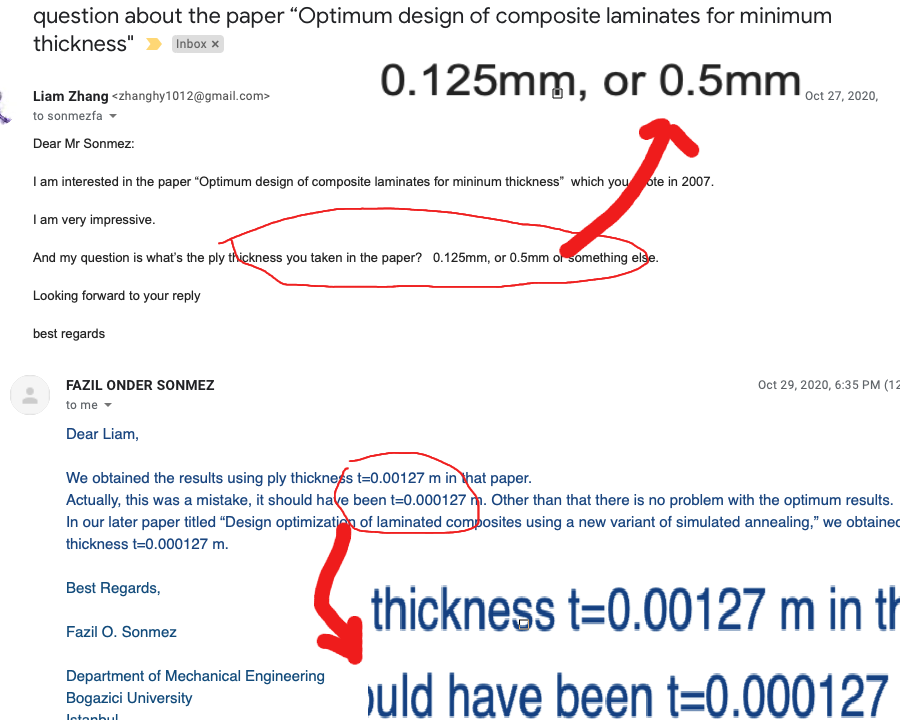
\includegraphics[width=1.0\linewidth]{2020-11-10-pre-image/email.png}
        \end{center}
    \end{column}
\end{columns}


\end{frame}
\begin{frame}{2. Methdology}
    \begin{columns}[c]
    \begin{column}{1\textwidth}
		\begin{itemize}
			\item modifying selection strategy: in order to handle the constraint search
			\item Self-adaptative mutation direction of fiber orientation and laminate thickness:
				random change the length, and the angle in the laminate.
			\item the self-adaptative parameters don't refer to parent's proportion, mutation
				probability.
		\end{itemize}
    \end{column}
    \begin{column}{0.8\textwidth}

    \end{column}

\end{columns}


\end{frame}

\begin{frame}{2. Self-adaptative GA: selection operator}
    \begin{columns}[c]
    \begin{column}{0.8\textwidth}
		\begin{itemize}
			\item acitve group: individual is used to increase the diversity of the population
			\item potential group: individual doesn't fulfill constraint
			\item proper group: individual meet constraint
		\end{itemize}
		
    \end{column}
\end{columns}
\end{frame}

\begin{frame}{2. Self-adaptative GA:  mutation operator}
    \begin{columns}[c]
    \begin{column}{1\textwidth}
		$\text{md} = [CT_1, \cdots, CT_{n-1}, CT_n] -  [ICV_0, \cdots, ICV_{n-1},
		ICV_n]$ \\
		\begin{itemize}
			\item  md means mutation direction.
			\item  $CT_i$ denotes the i-th constraint, such as weight, safety factor.
			\item  $ICV_i$ denotes individual's i-th constraint value, such as,  weight, safety
				factor of current individual.
		\end{itemize}

    \end{column}
\end{columns}
\end{frame}


\begin{frame}{2. Self-adaptative GA:  mutation operator}
    \begin{columns}[c]
	\begin{column}{1\textwidth}
		\begin{itemize}
			\item length mutation =  
				\[
				  \begin{cases}
					  LMC*[0, \sum_{i=1}^{N}{md_i}] & \text{if $\sum_{i=1}^{N}{md_i} > 0$} \\
					  LMC*[\sum_{i=1}^{N}{md_i}, 0] & \text{if $\sum_{i=1}^{N}{md_i} < 0$} \\
				  \end{cases}
				\] \\
				LMC stands for length mutation coefficient, it's a positive integer.
			\item angle mutation = 
				\[
				  \begin{cases}
					  AMC*[0, \sum_{i=1}^{N}{md_i}] & \text{if $\sum_{i=1}^{N}{md_i} > 0$} \\
					  AMC*[\sum_{i=1}^{N}{md_i}, 0] & \text{if $\sum_{i=1}^{N}{md_i} < 0$} \\
				  \end{cases}
				\] \\
				AMC stands for angle mutation coefficient, it's sign is unclear.
		\end{itemize}
	\end{column}
\end{columns}
\end{frame}



\begin{frame}{Result: Loading $N_x = 10, N_y=5 $ MPa m}
    \begin{columns}
    \begin{column}{0.5\textwidth}

        \begin{center}
            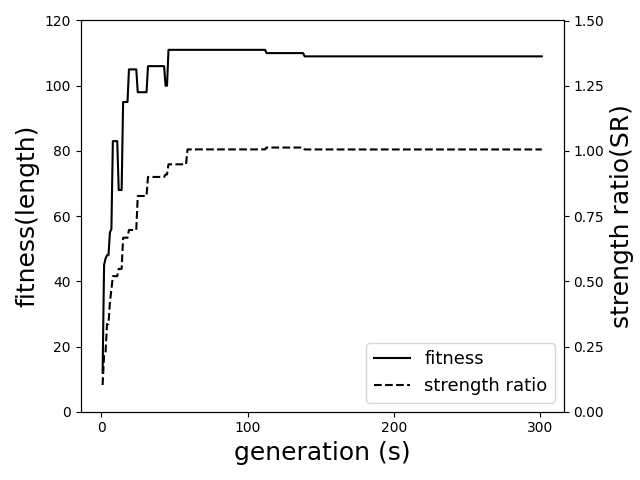
\includegraphics[width=1.0\linewidth]{2020-11-10-pre-image/two_distinct_angle_fitness_and_sr.png}
        \end{center}

        \begin{center}
              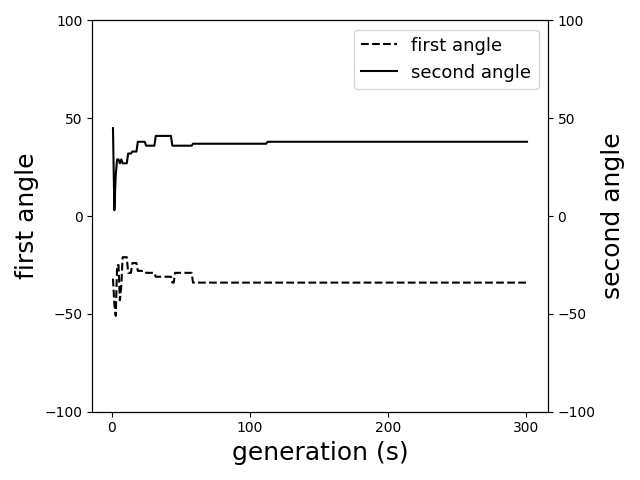
\includegraphics[width=1.0\linewidth]{2020-11-10-pre-image/two_distinct_angle_angle_change.png}
        \end{center}
    \end{column}
    \begin{column}{0.5\textwidth}
        \begin{center}
              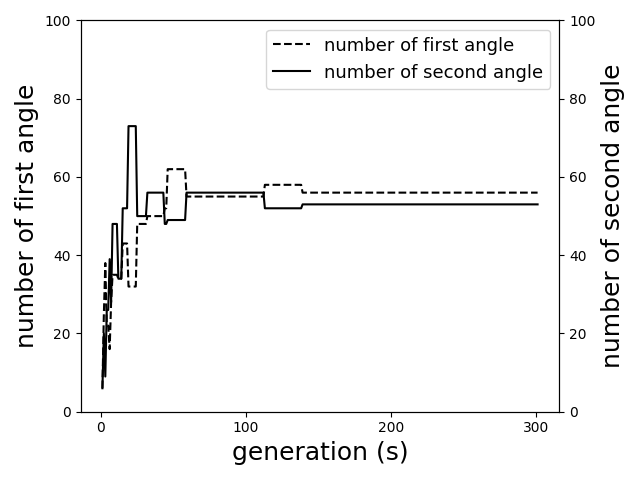
\includegraphics[width=1.0\linewidth]{2020-11-10-pre-image/two_distinct_angler_number_change.png}
              \captionof{figure}{Two distinct angles in the laminate}
        \end{center}
    \end{column}
\end{columns}
\end{frame}


\begin{frame}{Result: Loading $N_x = 10, N_y=5 $ MPa m}
    \begin{columns}
    \begin{column}{0.5\textwidth}

        \begin{center}
            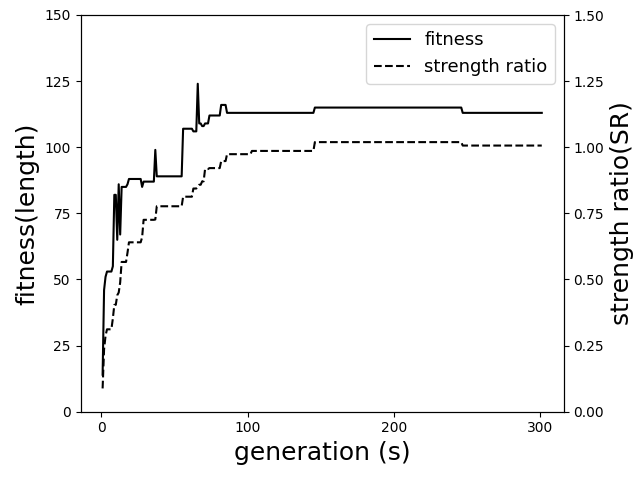
\includegraphics[width=1.0\linewidth]{2020-11-10-pre-image/Three_distinct_angles_fitness_and_sr.png}
        \end{center}

        \begin{center}
              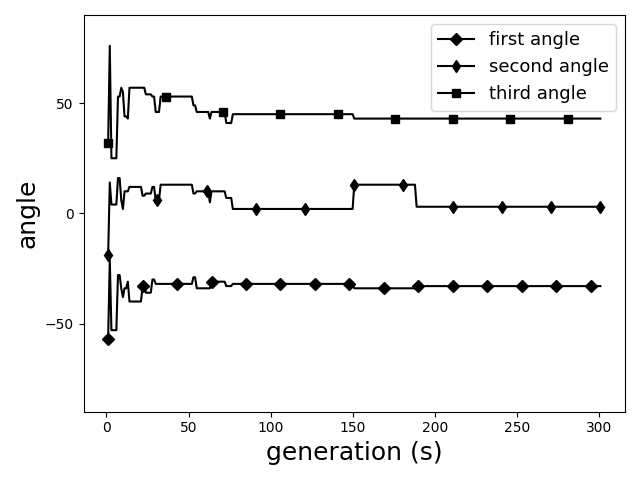
\includegraphics[width=1.0\linewidth]{2020-11-10-pre-image/three_distinct_angles_angle_change.png}
        \end{center}
    \end{column}
    \begin{column}{0.5\textwidth}
        \begin{center}
              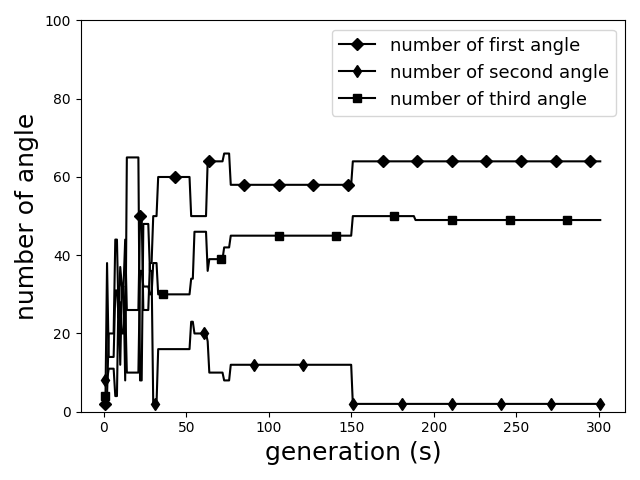
\includegraphics[width=1.0\linewidth]{2020-11-10-pre-image/three_distinct_angle_number_of_angle.png}
              \captionof{figure}{Three distinct angles in the laminate}
        \end{center}
    \end{column}
\end{columns}
\end{frame}



\end{document}
